\section{Method}
\label{sec:method}

\begin{strip}
  \centering
  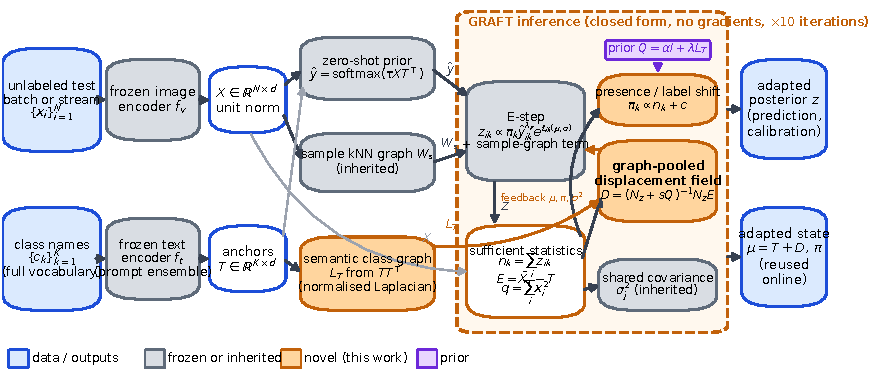
\includegraphics[width=\textwidth]{figures/fig1_framework.pdf}
  \captionof{figure}{\textbf{Overview of \method.} Frozen encoders produce unit-norm image features $X$ and text anchors $T$ (grey: frozen or inherited components; orange: this work). The text anchors define the zero-shot prior $\hat{y}$ and the semantic class graph $L_T$. Inference alternates a closed-form E-step over assignments $z$ with closed-form M-steps for the class proportions $\pi$ (presence), the graph-pooled displacement field $D$ and the shared covariance. The adapted prototypes are $\mu = T + D$; the posterior $z$ is the prediction. No gradient is computed and no parameter of the VLM is changed. In the online setting the sufficient statistics $(n, E, q)$ persist across batches.}
  \label{fig:framework}
\end{strip}

\subsection{Framework overview}
\method keeps the generative view of transduction~\cite{zanella2024transclip,zanella2025stata} but changes the object that is adapted: instead of $K$ independent prototypes it estimates a \emph{displacement field} $D\in\R^{K\times d}$ anchored at the text embeddings, $\mu_k = t_k + d_k$, with a prior that couples semantically related classes, together with the class proportions $\pi\in\Delta^K$ and a covariance shared by all classes. \Cref{fig:framework} shows the data flow: frozen encoders, the inherited sample graph $W_s$, the new class graph $L_T$, and a block-coordinate inference whose every step is closed form.

\subsection{Graph-regularized displacement field}
\label{sec:field}
\paragraph{Likelihood.}
Each class is a Gaussian with mean $\mu_k$ and a diagonal covariance $\Sigma=\diag(\sigma^2)$ shared across classes. As in TransCLIP, the likelihood is tempered by $\kappa$, which plays the role of a covariance inflation and keeps the responsibilities soft on $d$-dimensional features:
\begin{equation}
  \ell_{ik}(D,\sigma) = -\frac{1}{2\kappa}\Big[\sum_{j=1}^{d}\frac{(x_{ij}-t_{kj}-d_{kj})^2}{\sigma_j^2} + \sum_{j=1}^{d}\log\sigma_j^2\Big].
  \label{eq:lik}
\end{equation}

\paragraph{Prior.}
The field is given a Gaussian Markov random field prior~\cite{rue2005gmrf} that factorises over feature dimensions,
\begin{equation}
  p(D) \propto \exp\Big(-\tfrac{1}{2}\sum_{j=1}^{d} d_{:j}^{\top} Q\, d_{:j}\Big),\qquad
  Q = \frac{\alpha I_K + \lambda L_T}{\kappa\,\bar{\sigma}^2},
  \label{eq:prior}
\end{equation}
with $\bar{\sigma}^2 = \tfrac{1}{d}\sum_j\sigma_j^2$. The term $\alpha I_K$ pulls every displacement towards zero, that is, every prototype towards its text anchor; the term $\lambda L_T$ penalises the Dirichlet energy $\sum_{k\sim l} w_{kl}\|d_k/\sqrt{\mathrm{D}_k} - d_l/\sqrt{\mathrm{D}_l}\|^2$ and therefore asks the displacements of neighbouring classes to agree. Dividing by $\kappa\bar{\sigma}^2$ expresses $\alpha$ and $\lambda$ in units of sample counts: a prior strength of $\alpha=1$ is worth one tempered observation. Writing $N_z=\diag(n_1,\dots,n_K)$, $\bar{x}_k = \sum_i z_{ik}x_i/n_k$ and $e_k = \bar{x}_k - t_k$ (with $e_k=0$ when $n_k=0$), the maximum a posteriori field given the responsibilities is obtained for every feature dimension $j$ from a $K\times K$ linear system,
\begin{equation}
  d_{:j} = \big(N_z + s_j(\alpha I_K + \lambda L_T)\big)^{-1} N_z\, e_{:j}, \qquad s_j = \sigma_j^2/\bar{\sigma}^2 .
  \label{eq:dsolve}
\end{equation}
\Cref{eq:dsolve} is a graph filter applied to the empirical displacements, weighted by how much evidence each class has (\cref{fig:module}). Classes with $n_k \gg \alpha+\lambda$ keep their empirical displacement; classes with little or no evidence receive a smoothed combination of their neighbours' displacements. The $d$ systems share the matrix up to the scalar $s_j$ and are solved jointly by preconditioned conjugate gradients, or exactly for small $K$.

\begin{figure}[t]
  \centering
  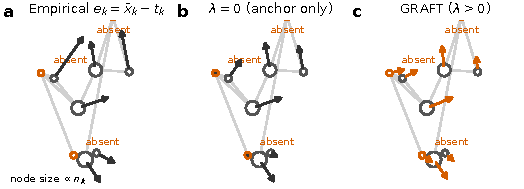
\includegraphics[width=\linewidth]{figures/fig2_module.pdf}
  \caption{\textbf{The graph-pooled displacement field} on a toy class graph (node size: soft count $n_k$). (a) Empirical displacements are noisy for rare classes and undefined for absent ones. (b) Independent shrinkage ($\lambda=0$) damps rare classes and leaves absent classes at their anchors. (c) With $\lambda>0$, \cref{eq:dsolve} transfers the displacement of well-observed classes along the graph; absent classes receive the harmonic extension of their neighbours (\cref{prop:absent}).}
  \label{fig:module}
\end{figure}

\subsection{Class presence as label shift}
\label{sec:presence}
The mixture weights $\pi$ are free parameters with a symmetric Dirichlet prior $\mathrm{Dir}(c+1)$. Their M-step is the smoothed count
\begin{equation}
  \pi_k = \frac{n_k + c}{N + Kc},
  \label{eq:pi}
\end{equation}
and they enter the E-step as $\log\pi_k$, which is the classical label-shift correction of a calibrated classifier~\cite{saerens2002adjusting}: the zero-shot posterior implicitly assumes uniform class priors, and \cref{eq:pi} replaces them by the estimate obtained from the batch. For a batch with $K_{\mathrm{eff}}\ll K$ classes, absent classes receive $\pi_k\approx c/(N+Kc)$ while present ones receive $n_k/(N+Kc)$; with $c=\tfrac{1}{2}$ a present class with sixteen samples is more than thirty times more likely a priori than an absent one in a batch of 64 over 1000 classes. The pseudo-count $c>0$ keeps $\log\pi_k$ finite and lets a class that was absent in earlier online batches re-enter the stream.

\subsection{Objective}
\label{sec:objective}
Collecting the terms, \method minimises over $(z, D, \sigma, \pi)$
\begin{align}
  J ={}& \sum_{i,k} z_{ik}\big[\log z_{ik} - \log\pi_k - \lambda_y\log\hat{y}_{ik} - \ell_{ik}(D,\sigma)\big] \nonumber\\
   &- \frac{\lambda_L}{2m_s}\sum_{i,i'} (W_s)_{ii'}\, z_i^{\top} z_{i'}
    + \frac{1}{2}\sum_{j} d_{:j}^{\top} Q\, d_{:j}
    - c\sum_k \log\pi_k ,
  \label{eq:objective}
\end{align}
where the first line is the variational free energy of the mixture with the text prior $\hat{y}^{\lambda_y}$ of~\cite{zanella2024transclip}, the second line contains the inherited sample-graph term ($m_s$ nearest neighbours), the new field prior and the presence prior. Setting $\lambda = 0$ and dropping the $\pi$ terms recovers the StatA objective up to its per-class covariances; setting in addition $\alpha=0$ and $\lambda_L = 0$ recovers the unanchored mixture.

\subsection{Inference}
\label{sec:inference}
\Cref{alg:batch} alternates four closed-form blocks. The E-step is the standard mean-field update with the Laplacian term linearised at the current $z$ (a majorise-minimise step~\cite{hunter2004mm,ziko2020laplacianshot,zanella2024transclip}):
\begin{equation}
  z_{ik} \propto \pi_k\,\hat{y}_{ik}^{\lambda_y}\exp\Big(\ell_{ik} + \frac{\lambda_L}{2m_s}\big[(W_s + W_s^{\top})z\big]_{ik}\Big),
  \label{eq:estep}
\end{equation}
iterated a few times. The M-steps are \cref{eq:pi}, \cref{eq:dsolve} and the shared variance $\sigma_j^2 = \tfrac{1}{N}\sum_{i,k} z_{ik}(x_{ij}-\mu_{kj})^2$. All quantities depend on the data only through the sufficient statistics $n = z^{\top}\mathbf{1}$, $S = z^{\top}X$ and $q = \sum_i x_i^{\odot 2}$, which makes the online variant immediate: statistics are accumulated over the stream with an optional forgetting factor $\varrho$, and the same M-steps are applied after every batch (algorithm in the supplementary material). The prediction for a batch is its posterior $z$ after adaptation, as in the transductive protocol of~\cite{zanella2025stata}; a strictly inductive variant predicts before the statistics are updated.

\begin{algorithm}[t]
\caption{\method, batch (transductive) inference}
\label{alg:batch}
\begin{algorithmic}[1]
\Require features $X\in\R^{N\times d}$, anchors $T\in\R^{K\times d}$, graph $L_T$, $(\alpha,\lambda)$ or empirical Bayes, $c$, $\kappa$, $\lambda_y$, $\lambda_L$
\State $\hat{y}\gets\mathrm{softmax}(\tau XT^{\top})$; $z\gets\hat{y}$; $D\gets 0$; $\pi\gets\mathbf{1}/K$; $\sigma^2\gets$ variance of $X$ about $T$ under $\hat{y}$
\State $W_s\gets$ $m_s$-NN cosine graph of $X$
\For{$t=1,\dots,T_{\max}$}
  \State E-step: update $z$ by \cref{eq:estep} ($n_{\mathrm{inner}}$ sweeps)
  \State $n\gets z^{\top}\mathbf{1}$;\; $\bar{X}\gets N_z^{-1}z^{\top}X$;\; $E\gets\bar{X}-T$ (rows with $n_k=0$ set to $0$)
  \State $\pi\gets(n+c)/(N+Kc)$ \Comment{presence}
  \State optionally $(\alpha,\lambda)\gets\argmax$ marginal likelihood of $E$ (\cref{sec:eb})
  \State $D\gets$ solution of \cref{eq:dsolve} \Comment{graph-pooled field}
  \State $\sigma_j^2\gets\tfrac{1}{N}\big[q_j - 2\sum_k\mu_{kj}S_{kj} + \sum_k n_k\mu_{kj}^2\big]$ with $\mu=T+D$
\EndFor
\State \Return $z$ (posterior), $(D,\pi,\sigma^2)$
\end{algorithmic}
\end{algorithm}



\subsection{Empirical Bayes selection of the pooling strength}
\label{sec:eb}
Fixed $(\alpha,\lambda)$ are used for all datasets in the main protocol, but the model also admits a label-free rule. Given the responsibilities, the empirical displacements of the present classes $P=\{k: n_k\ge 1\}$ are, under the model, $e_P = d_P + \epsilon$ with $\epsilon_k\sim\mathcal{N}(0,\kappa\sigma^2/n_k)$ and $d_P\sim\mathcal{N}(0,\tilde{Q}_P^{-1})$, where $\tilde{Q}_P$ is the Schur complement of $Q$ onto $P$. With the isotropic approximation $\sigma_j^2\approx\bar\sigma^2$ the marginal likelihood of $E_P$ is a Gaussian with covariance $C=\kappa\bar\sigma^2(\tilde{Q}_P^{-1}+N_{z,P}^{-1})$ per dimension,
\begin{equation}
  \log p(E_P\,|\,\alpha,\lambda) = -\tfrac{1}{2}\tr\big(E_P^{\top}C^{-1}E_P\big) - \tfrac{d}{2}\log\det C + \mathrm{const},
  \label{eq:evidence}
\end{equation}
which we maximise over a small logarithmic grid at every M-step whenever at least three classes are present (details in the supplementary material).

\subsection{Analysis}
\label{sec:analysis}
All proofs are short and given in the supplementary material; the statements are also verified numerically by the unit tests shipped with the code.

\begin{proposition}[Special cases]
\label{prop:special}
With $\lambda=0$, \cref{eq:dsolve} gives $d_k = \frac{n_k}{n_k+\alpha s_j}\,e_k$ per dimension, the count-based anchor shrinkage of StatA~\cite{zanella2025stata} (\cref{eq:stata}) and MOON~\cite{huang2026moon}. With $\alpha=0$, $L_T$ the Laplacian of the complete graph and $\lambda\to\infty$, every class receives the same displacement $d = \sum_k n_k e_k / \sum_k n_k$, the count-weighted mean displacement, that is, a single global shift of all prototypes.
\end{proposition}

\begin{proposition}[Absent classes are harmonic extensions]
\label{prop:absent}
Let $A=\{k: n_k = 0\}$ and $P$ its complement, and let $Q_\lambda = \alpha I + \lambda L_T$. The solution of \cref{eq:dsolve} satisfies $Q_{\lambda,AA}\,D_A + Q_{\lambda,AP}\,D_P = 0$, so $D_A = -Q_{\lambda,AA}^{-1}Q_{\lambda,AP}D_P$ is the harmonic extension of the present-class field, and $D_P$ solves \cref{eq:dsolve} restricted to $P$ with $Q_\lambda$ replaced by its Kron reduction $Q_\lambda/Q_{\lambda,AA}$~\cite{dorfler2013kron}. Adding absent classes to the vocabulary therefore changes the present-class prototypes only through the effective graph among them, never through data.
\end{proposition}

\begin{proposition}[Pooling never increases posterior variance]
\label{prop:variance}
Under the model of \cref{sec:field}, the posterior covariance of $d_{:j}$ given $z$ is $\kappa\sigma_j^2\,(N_z + s_j Q_\lambda)^{-1}$. Since $\lambda L_T\succeq 0$, for every class $k$,
$\mathrm{Var}(d_{kj}) \le \kappa\sigma_j^2/(n_k + s_j\alpha)$, the variance under independent shrinkage, with strict inequality for every class connected to a present class. For an absent class the bound under independent shrinkage is the prior variance $\kappa\sigma_j^2/(s_j\alpha)$, whereas with $\lambda>0$ it is reduced by the neighbours' counts.
\end{proposition}

\begin{proposition}[Monotone block updates]
\label{prop:monotone}
Each block update of \cref{alg:batch} is the exact minimiser of \cref{eq:objective} over its block when $\lambda_L=0$, so $J$ decreases monotonically and converges; with $\lambda_L>0$ the E-step minimises a majoriser of $J$, as in~\cite{zanella2024transclip}.
\end{proposition}

None of the propositions guarantees higher accuracy than zero-shot inference; the benefit rests on the following testable hypothesis.

\begin{hypothesis}[Class-level smoothness]
\label{hyp:smooth}
The oracle displacement field $e^{\star}_k = \E[x\,|\,y=k] - t_k$ has a Dirichlet energy on $L_T$ that is substantially smaller than on a random graph with the same degree sequence. If this fails, $\lambda L_T$ cannot help and \method reduces, in expectation, to the behaviour of anchor-only shrinkage.
\end{hypothesis}

\subsection{Complexity}
\label{sec:complexity}
Per outer iteration the E-step costs $O(NKd + N m_s K)$, the statistics $O(NKd)$, the presence update $O(K)$ and the field $O(n_{\mathrm{cg}}\,K d\,(1+m))$ with conjugate gradients ($O(K^3 + K^2 d)$ exactly). Memory is $O(NK + Kd + K^2)$; the class graph has $O(Km)$ edges and is built once per vocabulary. Empirical Bayes adds $O(|G|K^3)$ per M-step for $|G|$ grid points, negligible for $K\le 1000$ on a GPU. No backward pass is executed and the VLM is untouched after feature extraction.
